\documentclass[10pt]{extarticle}
\usepackage{amsmath}
\usepackage{amsfonts}
\usepackage{amssymb}
\usepackage{extsizes}
\usepackage{float}
\usepackage{graphicx}
\usepackage[margin = 1in]{geometry}
\usepackage{hyperref}
\usepackage[english]{babel}
\usepackage[backend=biber, style=numeric]{biblatex}
\usepackage[skins, minted]{tcolorbox}
\usepackage[T1]{fontenc}
\usepackage{lmodern}

\addbibresource{refs.bib}

\usepackage{minted}
\tcbset{listing engine=minted}
\tcbuselibrary{breakable}
\setminted{
	fontsize = \tiny, 
	breaklines,
	linenos = 1,
	numbersep = 2mm,
	autogobble,
	frame = none,
	style = friendly
}

\definecolor{rblue}{HTML}{75AADB}
\definecolor{stanred}{HTML}{B2001D}
\definecolor{jagsyellow}{HTML}{FFCB00}
\newtcbinputlisting{\tcbr}[1]{
	listing file = #1, 
	listing only, 
	minted language = R, 
	title = \lstinline{#1}, 
	minted options = 
	{
		fontsize = \scriptsize, 
		breaklines,
		linenos,
		numbersep = 2mm,
		frame = none,
		style = friendly,
		xleftmargin = 12pt
	}, 
	breakable,
	boxrule = 1pt,
	colback = white,
	colframe = rblue
}
\newtcbinputlisting{\tcbstan}[1]{
	listing file = #1, 
	listing only, 
	minted language = Stan, 
	title = \lstinline{#1}, 
	minted options = 
	{
		fontsize = \scriptsize, 
		breaklines,
		linenos,
		numbersep = 2mm,
		frame = none,
		style = friendly,
		xleftmargin = 12pt
	}, 
	breakable,
	boxrule = 1pt,
	colback = white,
	colframe = stanred
}
\newtcbinputlisting{\tcbjags}[1]{
	listing file = #1, 
	listing only, 
	minted language = R, 
	title = \lstinline{#1}, 
	minted options = 
	{
		fontsize = \scriptsize, 
		breaklines,
		linenos,
		numbersep = 2mm,
		frame = none,
		style = friendly,
		xleftmargin = 12pt
	}, 
	breakable,
	boxrule = 1pt,
	colback = white,
	colframe = jagsyellow
}
\usepackage{lstbayes}
%\usepackage[usenames,dvipsnames]{color}    

\newcommand{\E}{\mathbb{E}}
\newcommand{\Var}{\mathrm{Var}}
\renewcommand{\vec}[1]{\mathbf{#1}}
\newcommand{\Cov}{\mathrm{Cov}}


\begin{document}
	
\title{Bayesian Data Analysis Assignment 2}
\author{Benjamin Cox, S1621312}
\date{\vspace{-5ex}}
\maketitle

\section*{Question 1}

\begin{figure}[H]
	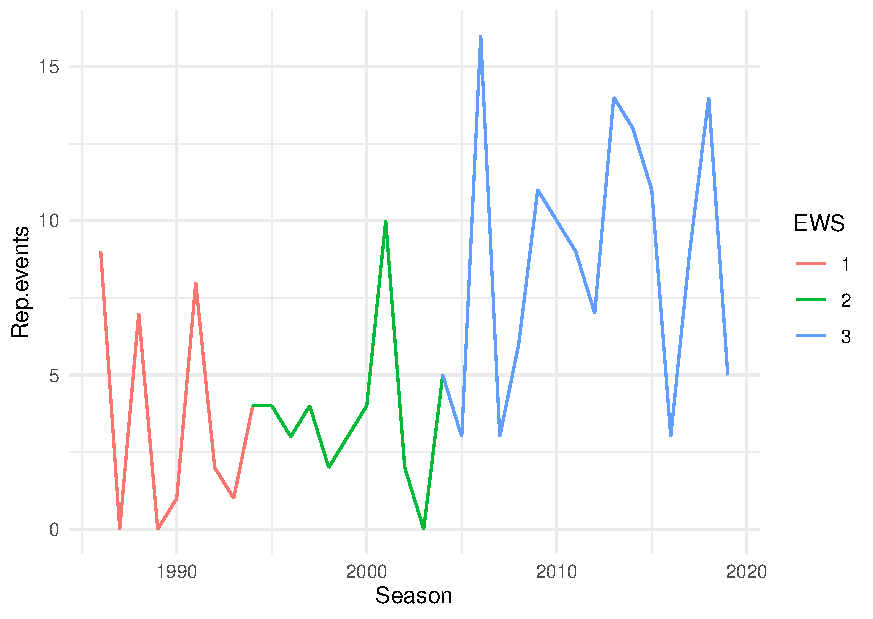
\includegraphics[width = 0.45\textwidth]{../ava_sea}
	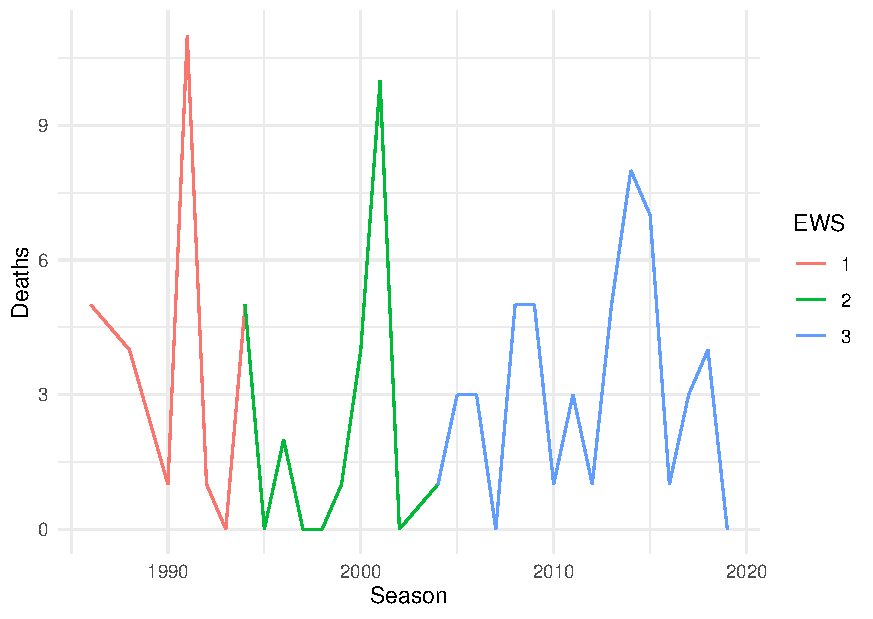
\includegraphics[width = 0.45\textwidth]{../dea_sea}
	\caption{Plots illustrating the temporal evolution of avalanche related statistics. The EWS measure is 1 = No EADS, 2 = EADS present, 3 = EADS online daily.}
	\label{fig:tempevava}
\end{figure}	

	From the above graphs we can see a positive trend in the number of avalanches and year, but no obvious trend in the number of deaths. We calculate the correlations between the number of deaths and the number of avalanches separated into EWS periods. 
	
	We obtain the following correlations (90\% bootstrap intervals)
\begin{table}[H]
	\centering
	\begin{tabular}{ccc}
		\hline
		No EADS & EADS & EADS Online \\
		\hline
		0.807 (0.9325, 0.9986) & 0.875 (0.1890, 0.9728) & 0.602 (0.3842, 0.8147) \\
		\hline
	\end{tabular}
\end{table}
This shows that the events become less correlated after the general public obtained easy access to EADS. It is not likely that the introduction of EADS increased to correlation, so the observed increase in correlation for that period is likely due to noise (10 events in 2001 resulting in 10 deaths). However it may also be due to an increase in user confidence, which led to foolish behaviour.

We are now going to model the number of deaths in avalanches. We are using a Poisson model with a logarithmic (canonical) link function. 

Our formulae are as follows:

\begin{align*}
\log(\lambda_i) &= \beta_0 + \beta_1\cdot \mathrm{Rep.events}_i + \beta_2 \cdot \mathrm{EADS1}_i + \beta_3 \cdot \mathrm{EADS2}_i\\
\mathrm{Deaths}_i &\sim \mathrm{Poisson}(\lambda_i)
\end{align*}

We note that these parameters have a multiplicative effect on the rate, so it is fine to have an intercept on physical terms. We will remove the intercept later.

We place wide normal priors on all $\beta_i$ and code up our model. The code is given in \ref{code:stan_1}, with a JAGS version given in \ref{code:jags_1}. 

We run it and obtain the following posterior summaries. We have exponentiated our parameters prior to summarising to ease interpretation.

\begin{table}[ht]
	\centering
	\begin{tabular}{rrrrr}
		\hline
		& (Intercept) & Rep.events & EADS1TRUE & EADS2TRUE \\ 
		\hline
		Min. & 0.41 & 1.07 & 0.28 & 0.12 \\ 
		1st Qu. & 1.08 & 1.17 & 0.66 & 0.32 \\ 
		Median & 1.32 & 1.19 & 0.81 & 0.39 \\ 
		Mean & 1.37 & 1.19 & 0.85 & 0.40 \\ 
		3rd Qu. & 1.60 & 1.22 & 0.99 & 0.47 \\ 
		Max. & 4.12 & 1.34 & 2.75 & 1.10 \\ 
		\hline
	\end{tabular}
\caption{Posterior summaries for the first Poisson model}
\label{tab:postsum_po}
\end{table}

From this we can make some initial conclusions. We see that the expected number of deaths increases by 1.19 times per avalanche (all other variables held constant). We also see that each EADS evolution decreases the expected number of deaths, by 0.85 and 0.40 times respectively. The latter is a rather large decrease, befitting of the drastic change in preparation tact that the EADS going online brought about.

We are interested in the posterior predictive distribution. We want to predict the probability of observing less than 15 deaths given 20 avalanches next year. We know that EADS will be online, so we have the appropriate data. 

We obtain a probability of $P(D<15|A=20, EADS=2) = 0.312$. This is roughly expected, as the number of avalanches increases deaths multiplicatively in expectation. In contrast the probability of less than 15 deaths for 10 avalanches is computationally indistinguishable from 1.

We are also interested in the probability of observing more than 1 death per avalanche in each stage of the EADS lifespan (not present, present, online). To do this we are going to have to make an assumption. We assume that the mean number of avalanches occurs. 

\printbibliography

\appendix

\section{Code for Question 1}
\subsection{R}
%\inputminted{R}{../Q1.R}
\tcbr{../Q1.R}
\tcbr{../jags/Q1jags.R}
\label{code:main_1}
\subsection{Stan}
\tcbstan{../stan/poisson_glm.stan}
\tcbstan{../stan/poisson_glm_exvar.stan}
\label{code:stan_1}
\subsection{JAGS}
\tcbjags{../jags/poisson.jags}
\tcbjags{../jags/poisson_exvar.jags}
\label{code:jags_1}
\section{Code for Question 2}
\subsection{R}
\tcbr{../Q2.R}
\label{code:main_2}
\subsection{Stan}
\tcbstan{../stan/binomial_glm.stan}
\tcbstan{../stan/binomial_glm_randomeffects.stan}
\label{code:stan_2}
\end{document}

